\chapter{Zukunft von DevOps}

DevOps ist ein neuer Ansatz und wird aktuell fast nur von den Innovatoren wie Netflix, Amazon und Google angewendet. Enterprise Unternehmen sind ebenfalls an continuous delivery und deployment interessiert und denken über den Einsatz von DevOps nach. Für Startup Unternehmen ist DevOps nicht von Bedeutung, da ihr Fokus auf Kundengewinnung liegt. Erst beim Wachsen des Unternehmens benötigen sie eine flexiblere Architektur, wie die DevOps anbietet. \\
Aufgrund der geringen Verbreitung sind die Vorteile von DevOps gegenüber der aufwendigen Einführung noch nicht eindeutig abzuschätzen. Erst sobald mehrere Unternehmen DevOps einführen, ist die Kluft überwunden und viele weitere Unternehmen entscheiden sich für die Einführen von DevOps. Abbildung X zeigt die Entwicklung der Einführung beispielsweise einer neuen Architektur. DevOps ist momentan dabei die Kluft (Chasm) zu überspringen. 

\begin{figure}[htbp]
  \centering
  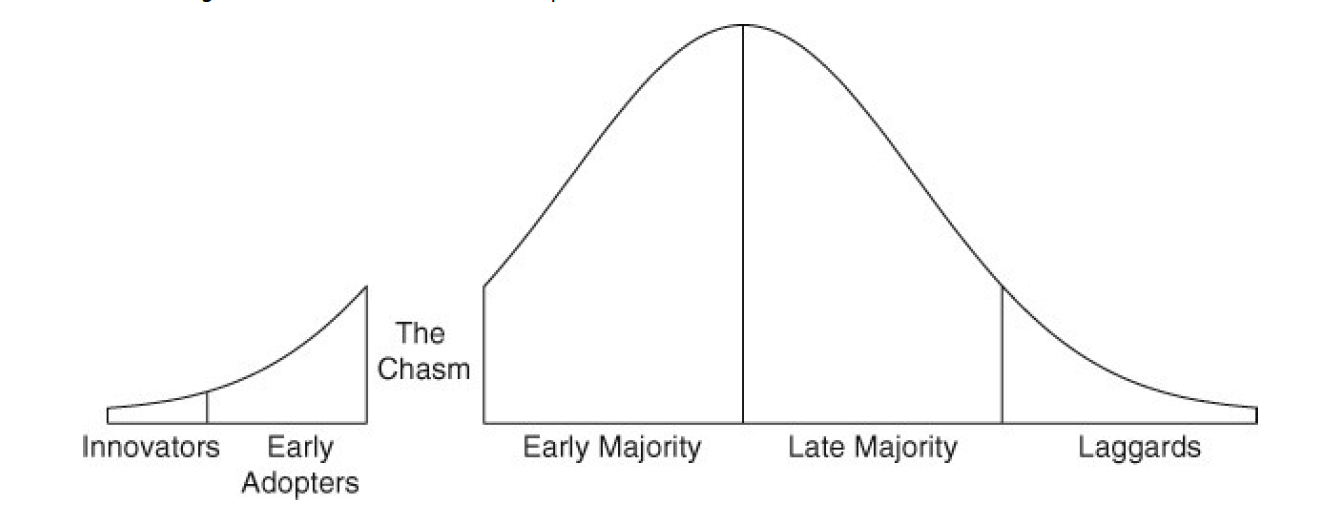
\includegraphics[width=0.5\textwidth]{pictures/chasm.png}
	\caption{Chasm}
	\label{Chasm}
\end{figure} 

Im folgenden wird auf einige Probleme und Anforderungen eingegangen, die DevOps mit sich bringen.

\section{Organisatorische Probleme}

\subsection{Stackholder mit Einfluss auf Dev und Ops}
DevOps versucht Dev und Ops zusammen zu führen um den Koordinationsaufwand zu verringern. Allerdings existieren einige Stackholder, die Einfluss auf Dev und Ops haben und Probleme verursachen.//

Businessverantwortliche haben großen Einfluss in den meisten Bereichen der Organisation. Neue Produkte oder Änderungen in der Versorgungskette haben Auswirkungen auf Dev und Ops. Durch kurze Entwicklungs- und Produktionsphasen bleibt nicht viel Zeit für die Koordination zwischen Businessverantwortlichen, Devs und Ops. Daher regelt der \textit{BizOps} die Koordination zwischen den drei Parteien.\\
Der Datenanalytiker betreibt mit Hilfe von beispielsweise Clustern Datenanalyse. Der gewonnene Einblick in das Business hilft Kundenverhalten zu verstehen und Bereiche für Optimierung zu finden.//
Der Sicherheitsprozess muss agile gehalten werden, um mit dem continuous deployment mitzuhalten. Dies ist nicht nur eine organisatorische Angelegenheit, sondern auch Abhängig der Sicherheitsprüfer.

\subsection{Verantwortung und Reorganisation}

Mircoservices werden von kleinen Teams verwaltet, allerdings von vielen anderen Teams aufgerufen. Sobald eine neue Version eines Services ausgeliefert wird, muss nicht nur sichergestellt werden, dass der Service andere Services korrekt benutzten kann, sondern auch dass andere Services den eigenen Service korrekt verwenden können. Eine Lösung dafür ist, dass Teams, die den neuen Service verwenden, bei der test suite Erstellung beteiligt sind. Sie sind also Co-Verantwortliche für den Service. 

\section{Prozess Probleme}
Durch die DevOps Praktiken entstehen auch eine vielzahl an Prozess Problemen. Es wird unter anderem für das Continuous Deployment eine so genannte Continuous Deployment Pipeline benötigt. Eine solche Pipeline besteht aus einer Vielzahl von Werkzeugen und ist dafür gedacht, den Programmcode auf eine Plattform zu deployen. Jedes dieser Werkzeuge kann allerdings eine Abhängigkeit zu dem Hersteller des Werkzeuges zur Folge haben, was die Portierbarkeit der Anwendung erschwert. Eine Möglichkeit solche Abhängigkeiten zu verhindern besteht darin bei dem Deployment auf gängige Standards zu setzen. Derzeit existieren allerdings noch keine akzeptierten Standards für die Werkzeuge innerhalb einer Continuous Deployment Pipeline. Durch eine höhere Verbreitung von DevOps, könnten in naher Zukunft tatsächlich Standards beschlossen werden. \\
Es existieren dennoch Strategien, um das Problem der Herstellerabhängigkeit zu minimieren. Zum einen sollte bei der Entwicklung auf einen defensiven Entwicklungsstil gepocht werden. Zum anderen existieren für eine Vielzahl von Werkzeugen Migrationswerkzeuge auf andere Werkzeuge. Diese Migrationswerkzeuge funktionieren allerdings nur bedingt gut und der Erfolg einer Migration hängt davon ab, ob nur eine Obermenge an Funktionen beider Werkzeuge verwendet wird. \\
Ein weiteres Prozess Problem, das durch die DevOps Praktiken entsteht, ist eng mit der Häufigkeit der Deployments verbunden. Eine gut funktionierende Deployment Pipeline ermöglicht häufigere Deployments. Dies bringt eine diverse Herausforderungen mit sich. Zunächst muss die Zeit zum Testen der Anwendung verringert werden. Dies kann zur Folge haben, dass Fehler nicht rechtzeitig entdeckt werden. Daher muss ein Rollback auf eine vorherige Version bei einem Fehler möglich sein. Der Fehler könnte mit dem darauf folgenden Deployment behoben sein. Zusätzlich muss eine automatische Fehlererkennung Bestandteil der Anwendung sein, damit bei Eintreten eines Fehlers automatisch ein Rollback stattfinden kann. \\
Durch häufigeres Deployment sind Unternehmen in der Lage, in kurzer Zeit viele neue Services anzubieten, was sowohl das Verhalten der Nutzer als auch die Last auf verschiedenen Services verändern kann. Zusätzlich kann auch das Deployment in eine Umgebung fäschlicherweise zu einem Alarm innerhalb eines Monitoring Tools der Umgebung führen. \\
All dies hat zur Folge, dass Unternehmen, die DevOps einsetzen, die Art ihres Monitorings und ihrer Qualitätssicherung verändern müssen.

\section{Technologische Probleme}
In der Regel sind die Werkzeuge einer Continuous Deployment Pipeline durch Skripte zur Integration miteinander verbunden. Um weitere Werkzeuge einzufügen bedarf es einer Änderung dieser Skripte. Dieser Ansatz bringt einve Vielzahl an Problemen mit sich. Es wird durch die Skripte schwerer nachvollziehbar, welche Komponenten auf welche Plattform deployed werde. Zusätzlich enthalten Services in der Regel keine Informationen mit welchen Werkzeugen sie deployed wurden. Daher wird eine Fehleranalyse bei einem korrupten Deployment erschwert.\\
Ein weiteres Problem entsteht dadurch, dass die Werkzeuge häufig die Sicherheitsinformationen wie Nutzername und Passwort von einem Werkzeug zum nächste weitergeben müssen und dadurch die Sicherheit gefährdet wird. \\
Das größte Problem besteht allerdings darin, dass viele Werkzeuge an sich nicht für Continuous Deployment geeignet sind, da diese in einer Zeit vor dem Continuous Deployment entstanden sind. Daher lassen sich neue Konzepte nur schwer auf diese Werkzeuge übertragen.